\documentclass[aspectratio=169,t,xcolor=table]{beamer}
\usepackage[utf8]{inputenc}


\usepackage[table]{xcolor}
\usepackage{booktabs} 
\usepackage{subcaption}

\usetheme{Ufg}

%-------------------------------------theorems--------------
\newtheorem{conj}{Conjetura}
\newtheorem{defi}{Definição}
\newtheorem{teo}{Teorema}
\newtheorem{lema}{Lema}
\newtheorem{prop}{Proposição}
\newtheorem{cor}{Corolário}
\newtheorem{ex}{Exemplo}
\newtheorem{exer}{Exercício}

\setbeamertemplate{theorems}[numbered]
\setbeamertemplate{caption}[numbered]

%-------------------------------------------------------------%
%----------------------- Primary Definitions -----------------%

% This command set the default Color, is also possible to choose a custom color
\setPrimaryColor{UFGBlue} 

% First one is logo in title slide (we recommend use a horizontal image), and second one is the logo used in the remaining slides (we recommend use a square image)
\setLogos{lib/logos/infw.png}{lib/logos/infw2.png} 


% -------------------------------------- Title Slide Information
\begin{document}
\title[Inf UFG]{Apresentações Instituto de informática}
\subtitle{Template Latex}

\author{Altino Dantas\inst{1} \and Deuslirio Junior\inst{2}}

\institute[UFG] % (optional)
{
  \inst{1}%
  Instituto de Informática\\
  Federal University of Goiás
  \and
  \inst{2}%
  Instituto de Informática\\
  Federal University of Goiás
}
\date{2019}
%-----------------------The next statement creates the title page.
\frame[noframenumbering]{\titlepage}


%------------------------------------------------Slide 1
\setLayout{vertical} % This command define the layout. 'vertical' can be replace with 'horizontal', 'blank, 'mainpoint', 'titlepage'

\begin{frame}
    \frametitle{Table of Contents}
    \tableofcontents
\end{frame}
%---------------------------------------------------------


%---------------------------------------------------------Slide 2
\section{Common presentation elements}

\subsection{Box}

\setLayout{vertical}
\begin{frame}{Example on using box}

    \footnotesize
    
    \begin{ex}
        Em uma versão da linguagem BASIC, o nome de uma variável é uma sequência de um ou dois caracteres alfanuméricos, em que letras maiúsculas e minúsculas não são distinguidas. Além disso, um nome de variável deve começar com uma letra e deve ser diferente das cinco sequências de dois caracteres reservadas para o uso de comandos. Quantos nomes diferentes de variáveis são possíveis nesta versão do BASIC?
    \end{ex}
    
    \begin{block}{Solução}
        Pela regra da soma, $V=V_1+V_2$. Como as variáveis só podem começar com letras, temos que $V_1=26$. Pela regra do produto, há $26\cdot 36=936$ sequências de tamanho $2$ que comecem com uma letra e terminam com um caracter alfanumérico. Porém, não se deve usar $5$ variáveis reservadas. Assim, $V_2=26\cdot 36-5=931$. Logo, há $V=V_1+V_2 = 26+931=957$ nomes diferentes para variáveis nesta versão do BASIC.
    \end{block}

\end{frame}
%---------------------------------------------------------


%--------------------------------------------------------- Slide 3
\subsection{Table}

\begin{frame}{Example on using table}

    \begin{table}[]
        \centering
        \caption{\label{tab:1}Countries and their codes}
        
        \renewcommand{\arraystretch}{1.5}
        \setlength{\tabcolsep}{10pt}
        
        {\rowcolors{2}{}{LightGray!10}
            \begin{tabular}{ p{3cm}p{3cm}p{3cm}  }
                \toprule 
                \textbf{Country Name} & \textbf{Code 2} & \textbf{Code 3} \\
                \midrule
                Afghanistan & AF &AFG \\
                Aland Islands & AX   & ALA \\
                Albania &AL & ALB \\
                Algeria    &DZ & DZA \\
                \bottomrule
            \end{tabular}
        }
    \end{table}
    
\end{frame}
%---------------------------------------------------------

\subsection{Image}

%--------------------------------------------------------- Slide 4
\begin{frame}{Example on using image}

    \begin{figure}
        \centering
        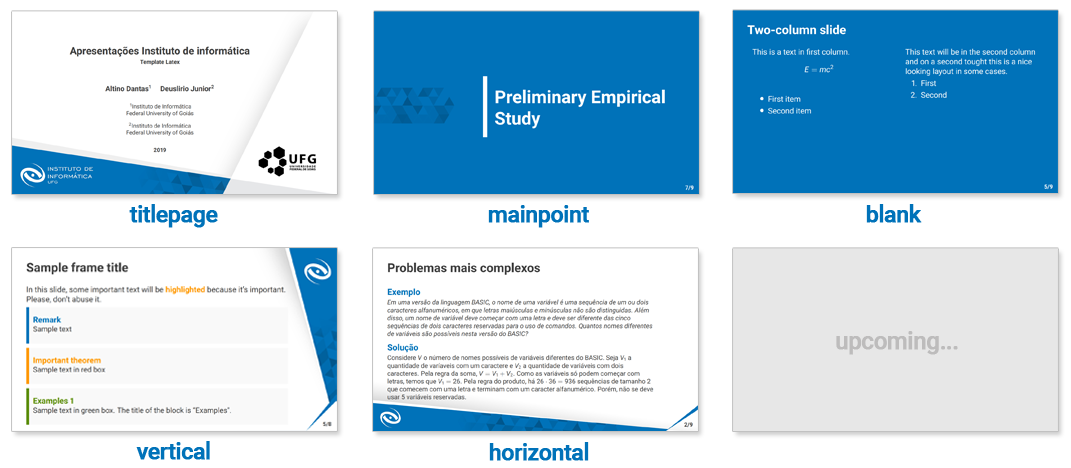
\includegraphics[width=.9\textwidth]{readme/layouts.png}
        \caption{Template's Layouts.}
        \label{fig:layouts}
    \end{figure}
    
\end{frame}
%---------------------------------------------------------


%--------------------------------------------------------- Slide 5
\section{Changing colors and Layouts}

\setLayout{blank} % Example of changing layout
\setBGColor{DarkOrange}  %Example of changing background color 

\begin{frame}{Clean layout and two-column text}
    
    \begin{columns}
    
        \column{0.5\textwidth}
        This is a text in first column.
        $$E=mc^2$$
        \begin{itemize}
        \item First item
        \item Second item
        \end{itemize}
        
        \column{0.5\textwidth}
        This text will be in the second column
        and on a second tought this is a nice looking
        layout in some cases.
        
        \begin{enumerate}
            \item First
            \item Second
        \end{enumerate}
        
    \end{columns}
    
\end{frame}
%---------------------------------------------------------


%---------------------------------------------------------Slide 6
%Highlighting text
\setLayout{vertical}
\begin{frame}{Sample frame title}
    
    In this slide, some important text will be
    \alert{highlighted} because it's important. Please, don't abuse it.
    
    \begin{block}{Remark}
        Sample text
    \end{block}
    
    \begin{alertblock}{Important theorem}
        Sample text in alert box
    \end{alertblock}
    
    \begin{examples}
        Sample text in green box. The title of the block is ``Examples".
    \end{examples}
    
\end{frame}
%---------------------------------------------------------


%---------------------------------------------------------Slide 7
\section{Main point layout}

\setLayout{mainpoint}
\setBGColor{DarkPurple}
\begin{frame}{}
    \frametitle{Preliminary Empirical Study}
\end{frame}
%-------------------------------------------------------


%---------------------------------------------------------Slide 8

\setLayout{horizontal}
\begin{frame}
    \frametitle{Sample frame title}
    This is a text in second frame. For the sake of showing an example.
    
    \begin{itemize}
        \item<1-> Text visible on slide 1
        \item<2-> Text visible on slide 2
        \begin{itemize}
            \item text subitem
        \end{itemize}
        \item<3> Text visible on slides 3
        \item<4-> Text visible on slide 4
    \end{itemize}
\end{frame}
%---------------------------------------------------------

\section{Thanks slide}
%---------------------------------------------------------Slide 9
\setLayout{blank}
\begin{frame}
    \centering
    \vspace{2cm}
    
    \textbf{\Huge Thanks}
    
    \ \\
    
    \textbf{Doubts and Suggestions}
    \ \\
    
    \text{\footnotesize altinodantas@gmail.com or deuslirio.junior@gmail.com}
    
    \vspace{2cm}
    \begin{figure}
        \centering
        \begin{subfigure}{0.2\textwidth}
            \centering
            
\includegraphics[height=1cm]{lib/logos/infw.png}
        \end{subfigure}%
        \qquad 
        \begin{subfigure}{0.2\textwidth}
            \centering
            
\includegraphics[height=1cm]{lib/logos/ufgw.png}
        \end{subfigure}
      
    \end{figure}
    
\end{frame}

%---------------------------------------------------------Slide 10
\setLayout{titlepage}
\setBGColor{DarkGray}
\titlepage
%-------------------------------------

\end{document}